\begin{figure}[H]
    \centering
    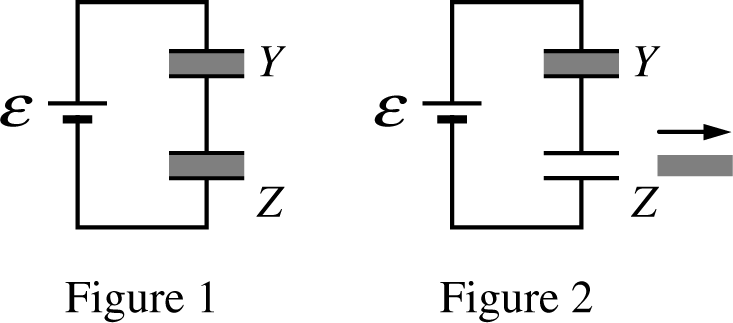
\includegraphics[scale=0.25]{images/img-014-040.png}
\end{figure}

% Multiple Choice Question 33
\begin{questions}\setcounter{question}{32}\question
Two identical capacitors, Y and Z, are connected in series with an ideal battery, as shown in figure 1 above, and fully charged. Each capacitor has a dielectric slab of dielectric constant $\kappa > 1$ between its plates. If the dielectric slab is removed from capacitor $Z$, which of the following describes what happens to the voltage across each capacitor?

\tabto{0.75cm} Voltage across
\tabto{5.00cm} Voltage across\\
\tabto{0.75cm} \underline{Capacitor $Y$}
\tabto{5.00cm} \underline{Capacitor $Z$}

\begin{choices}
\choice Increases        \tabto{4.25cm} Decreases
\choice Increases        \tabto{4.25cm} Increases
\choice Remains the same \tabto{4.25cm} Remains the same
\choice Decreases        \tabto{4.25cm} Decreases
\choice Decreases        \tabto{4.25cm} Increases
\end{choices}\end{questions}
